In Chapter \ref{ch:metacasanova} and \ref{ch:languages} we have presented the Metacasanova metacompiler and its meta-language and shown how to implement with it a small imperative language, C-{}-, and a DSL for game development, Casanova. The performance analysis showed that, although the development effort for the language compilers was greatly reduced by using Metacasanova, this has come to the cost of performance. The performance decay is due to the fact that the meta-type system of Metacasanova is unaware of the type system of C-{}- or Casanova. This requires all the type checking and access to data structures being performed at runtime, thus making a statically-typed language exhibit the behaviour and performance of dynamically typed languages. In this Chapter we propose a language extension \cite{DiGiacomo2017SLE} for Metacasanova that is thought to overcome the problem of performance decay and dynamic checks. In this context we use the term \textit{embedded language} to refer to a language that is being implemented in Metacasanova and \textit{embedded program} for a program implemented in an embedded language.

\section{Language extension idea}
\label{sec:ch_functors_idea}
The experimental results from Chapter \ref{ch:languages} showed that the performance of Metacasanova is strongly affected by the dynamic type checks and symbol table access at runtime. This is due to the fact that Metacasanova generates the code necessary to evaluate the semantics of accessing the value of a variable in the symbol table that mimics the behaviour of rules in natural semantics, but such evaluation is performed at runtime. However the runtime evaluation is only due to the limitations of the language presented so far, which is not able to build a symbol table while while compiling the meta-program, since

\begin{enumerate}
	\item The symbol table of a statically-typed language does not grow at runtime because it is built during the compilation.
	\item The position of an entry for a variable in the symbol table does not change during the program execution, thus every time we perform an access to the same variable, we access the very same element in the symbol table.
\end{enumerate}

\noindent
Analogously type checking in a statically-typed language is performed at compilation time rather than at runtime, which is a behaviour typical of dynamic languages such as Python. Metacasanova is forced to do runtime type checking because, at compilation time, the metacompiler only checks for the meta-types, i.e. the types of the language abstractions defined in the meta-language, but not for the program structures of the embedded program itself. This would require to be able to embed the type system of the embedded language into the meta-type system of Metacasanova. In this way the type checker of Metacasanova would be able to check at the same time the types of both the meta-program and of the embedded program. 

To better clarify what stated so far we show in the following section an example of what happens when accessing the field of a Casanova entity with the implementation given in Chapter \ref{ch:languages}. We then proceed to show the idea of a possible solution to overcome the performance decay.

\subsection{Field access in Casanova}
\label{subsec:ch_functors_casanova_example}
As we showed in Section \ref{subsec:ch_mcnv_languages_casanova_semantics}, an entity in Casanova embedded in Metacasanova is represented through a map where the key is the field name and the value is the value currently stored in the field. This representation is very similar to that of records or classes. Let us consider the following entity representing a physical body consisting of a \texttt{Position} and a \texttt{Velocity} in a 2D space:

\begin{lstlisting}
type PhysicalBody = {
  Position        : Vector2
  Velocity        : Vector2
}
\end{lstlisting}

\noindent
and the following rules for \texttt{PhysicalBody}

\begin{lstlisting}
rule Position = Position + Velocity * dt

rule Position =
  if Position.X > 500f then
    yield new Vector2(500f,Position.Y)
  elif Position.X < 0f then
    yield new Vector2(0f,Position.Y)
  elif Position.Y < 0f then
    yield new Vector2(Position.X,0f)
  elif Position.Y > 500f then
    yield new Vector2(Position.X,500f)
\end{lstlisting}

The first rule simply updates the position using the Euler approximation of the differential equation for the velocity

\begin{equation*}
v(t) = \dfrac{ds(t)}{dt}
\end{equation*}

\noindent
while the second rule ensures that the physical body does not exit a specific area, which could represent the playable area in a 2D game.

Assuming that the physical body is in position $(10,10)$, it is represented in Metacasanova through a map as shown in Table \ref{tab:ch_functors_physical_body}.

\begin{table}
	\centering
	\begin{tabular}{|c|c|}
		\hline
		\textbf{Field} & \textbf{Value} \\
		\hline
		Position	& 10 \\
		\hline
		Velocity & 10 \\
		\hline
	\end{tabular}
	\caption{Meta-representation of the physical body}
	\label{tab:ch_functors_physical_body}
\end{table}

\noindent
The Metacasanova semantics rule that evaluates the first Casanova rule will evaluate the expression in its body by accessing respectively the field \texttt{Position} and \texttt{Velocity} to compute the expression value. It then stores the expression value in \texttt{Position} as shown in Table \ref{tab:ch_functors_physical_body_access1_1}.

\begin{table}
	\centering
	\begin{tabular}{c|c|c|}
		\cline{2-3}
		& \textbf{Field} & \textbf{Value} \\
		\cline{2-3}
		$\Rightarrow$ & \cellcolor{green}{Position}	& \cellcolor{green}{10,10} \\ 
		\cline{2-3}
	  & Velocity & 10,0 \\
		\cline{2-3}
	\end{tabular}
	
	\vspace{0.15cm}
	\begin{tabular}{c|c|c|}
		\cline{2-3}
		& \textbf{Field} & \textbf{Value} \\
		\cline{2-3}
	  & Position	& 10,10 \\ 
		\cline{2-3}
		$\Rightarrow$ & \cellcolor{green}{Velocity} & \cellcolor{green}{10,0} \\
		\cline{2-3}
	\end{tabular}
	
	\vspace{0.15cm}
	\begin{tabular}{c|c|c|}
		\cline{2-3}
		& \textbf{Field} & \textbf{Value} \\
		\cline{2-3}
		$\Rightarrow$ & \cellcolor{green}{Position}	& \cellcolor{green}{11,10} \\ 
		\cline{2-3}
		& Velocity & 10,0 \\
		\cline{2-3}
	\end{tabular}

	\caption{Memory access in the first rule of the Physical Body. We assume \texttt{dt = 0.1} and \texttt{Velocity = (10,0)}}
	\label{tab:ch_functors_physical_body_access1_1}
\end{table}

\begin{table}
	\centering
	\begin{tabular}{c|c|c|}
		\cline{2-3}
		& \textbf{Field} & \textbf{Value} \\
		\cline{2-3}
		$\Rightarrow$ & \cellcolor{green}{Position}	& \cellcolor{green}{\fbox{501},10} \\ 
		\cline{2-3}
		& Velocity & 10,10 \\
		\cline{2-3}
	\end{tabular}
	
	\vspace{0.15cm}
	\begin{tabular}{c|c|c|}
		\cline{2-3}
		& \textbf{Field} & \textbf{Value} \\
		\cline{2-3}
		$\Rightarrow$ & \cellcolor{green}{Position}	& \cellcolor{green}{501,\fbox{10}} \\ 
		\cline{2-3}
		& Velocity & 10,10 \\
		\cline{2-3}
	\end{tabular}
	
	\vspace{0.15cm}
	\begin{tabular}{c|c|c|}
		\cline{2-3}
		& \textbf{Field} & \textbf{Value} \\
		\cline{2-3}
		$\Rightarrow$ & \cellcolor{green}{Position}	& \cellcolor{green}{500,10} \\ 
		\cline{2-3}
		& Velocity & 10,10 \\
		\cline{2-3}
	\end{tabular}
	\caption{Memory access in the second rule of the Physical Body. We assume \texttt{Position.X = 501}}
\end{table}

\noindent
As for the second rule, assuming that \texttt{Position.Y > 500f}, the rule will access \texttt{Position} three times: (\textit{i}) to evaluate the expression in the conditional, (\textit{ii}) to read \texttt{Position.Y} when instantiating a new vector, and (\textit{iii}) to write the new vector in \texttt{Position}. This situation is shown in Table

It should now appear clear that every time we need to read or write \texttt{Position} we access the first element of the table, while for \texttt{Velocity} we always access the second. In the following snippet we provide an alternative version of the code for the Casanova rules above that shows what really happens in Casanova embedded in Metacasanova :

\begin{lstlisting}
rule Position = PhysicalBodyTable[0] + PhysicalBodyTable[1] * dt
  
rule Position =
	if PhysicalBodyTable[0].X > 500f then
		yield new Vector2(500f,PhysicalBodyTable[0].Y)
	elif PhysicalBodyTable[0].X < 0f then
		yield new Vector2(0f,PhysicalBodyTable[0].Y)
	elif PhysicalBodyTable[0].Y < 0f then
		yield new Vector2(PhysicalBodyTable[0].X,0f)
	elif PhysicalBodyTable[0].Y > 500f then
		yield new Vector2(PhysicalBodyTable[0].X,500f)
\end{lstlisting}

Let us now assume that the program provides an invalid value for the update of \texttt{Position}:

\begin{lstlisting}
rule Position = "(10,10)"
\end{lstlisting}

\noindent
what would happen in embedded Casanova is that the type checker evaluates the type of the expression in the rule body, obtaining \texttt{string}. This type is then compared with that of \texttt{Position}, which is \texttt{Vector2}, and at this point an error would be reported. Again, this would require at runtime to access the first element of a symbol table containing type information about the entity fields. Note that all these lookups are not array accesses but rather dictionary accesses.

\subsection{Inlining the entity fields}
\label{subsec:ch_functors_inlining}
From the example above we can notice that, when the program runs, the symbol table used to represent a Casanova entity does not change, nor its entries change position. This means that every time we read or write the same field we perform the same access in the table. In the implementation provided in Section \ref{subsec:ch_mcnv_languages_casanova_semantics} this access requires to evaluate a Metacasanova rule that is able to traverse the dictionary used for the entity symbol table and return the stored value. The traverse is performed every time, regardless of the fact that the field we are trying to access is indeed the same. Moreover, as it was also stated in Section \ref{ch:mcnv_languages_evaluation}, we are looking at the very optimistic scenario where we make use of external .NET dictionaries to actually model the entity. If one had to rely solely on language abstractions defined in Metacasanova the symbol table should be modelled as a list of pairs containing field names, represented as strings, and meta-data structures representing values in the embedded language, introducing even a greater overhead. The physical body modelled in such way would then look like

\begin{lstlisting}
[("Position",(10,10)),("Velocity",(10,0)]
\end{lstlisting}

Accessing \texttt{Position} would then be performed by a Metacasanova rule that looks for the correct field name and stops when the field in this tuple has been reached:

\begin{lstlisting}
name = fieldName
----------------------------------
getField name ((fieldName,value) :: t) -> value

name <> fieldName
getField name t -> v
----------------------------------
getField name ((fieldName,value) :: t) -> v
\end{lstlisting}

\noindent
However the traversal of the tuple would always be the same when looking for a specific field, namely for \texttt{Position} the first Metacasanova rule will always be executed, while for \texttt{Velocity} the first time the second rule will be executed, which in turn recursively evaluates the remaining part of the list. The recursive call will then trigger the first rule at the second step. That being said, since the table does not grow and the access patterns are always the same, we could represent an entity as a nested tuple of pairs, in the fashion of Church encoding \cite{pierce2002types, kleene1935theory}, and inline in the code \texttt{fst PhysicalBodyTable} for \texttt{Position} and \texttt{fst(snd PhysicalBodyTable)} for \texttt{Velocity} whenever we require to access the respective fields, without repeating the same traversal every time. In this way the entity would look like:

\begin{lstlisting}
PhysicalBodyTable = ("Position",(10,10)),(("Velocity",(10,0)),())
\end{lstlisting}

\noindent
and thus \texttt{fst PhysicalBodyTable} (access to \texttt{Position}) would return\\ \texttt{("Position",(10,10))} and \texttt{fst(snd PhysicalBodyTable)} (access to\\ \texttt{Velocity}) would return \texttt{("Velocity",(10,0))}.

In the following sections we present the language extension required to allow this form of inlining and we show their usage implementing the example above.

\section{Modules and Functors}
\label{sec:ch_functors_modules_functors}
In order to implement the idea about inlining symbol table access and embed the type system of a language inside Metacasanova type system we extend the language with \textit{functors} and \textit{modules}. Functors are a concept borrowed form category theory that here are used in a more narrow sense. Formally a category is defined as follows \cite{asperti1991categories, mitchell1965theory, pierce1991basic}:

\begin{definition}
	A category $\mathcal{C}$ is made of
	
	\begin{itemize}[noitemsep]
		\item A collection of \textit{objects}.
		\item A collection of \textit{arrows} or \textit{morphism} between objects. Each morphism starts from a source object and ends into a target object.
		\item For every triplet of objects, there exists a composition operation $\circ$, such that, given the morphisms $f:a \rightarrow b$ and $g:b \rightarrow c$ then $g \circ f: a \rightarrow c$.
		\item The composition operation is associative, i.e. $f \circ (g \circ h) = (f \circ g) \circ h$.
		\item For each object $x$ There exists a morphism $1_x: x \rightarrow x$, called \textit{identity}, such that for every morphism $f:a \rightarrow x$ and $g: x \rightarrow b$ we have that $f \circ 1_x = f$ and $g \circ 1_x = g$.
	\end{itemize}
\end{definition}

\noindent
Functors are mapping between two categories defined as follows:

\begin{definition}
	Given two categories $\mathcal{C}_1$ and $\mathcal{C}_2$, a \textit{functor} $\mathcal{F}$ from $\mathcal{C}_1$ to $\mathcal{C}_2$ is a mapping such that:
	
	\begin{itemize}
		\item Each object $x$ of $\mathcal{C}_1$ is mapped to an object $\mathcal{F}(x)$ of $\mathcal{C}_2$.
		\item Each morphism $f: a \rightarrow b$ of $\mathcal{C}_1$ is mapped to a morphism $\mathcal{F}(f): \mathcal{F}(a) \rightarrow \mathcal{F}(b)$ such that
		\begin{itemize}
			\item $\mathcal{F}(1_x) = 1_{\mathcal{F}(x)}$.
			\item For all morphism $f: a \rightarrow b$ and $g: b \rightarrow c$ of $\mathcal{C}_1$ we have that $\mathcal{F}(g \circ f) = \mathcal{F}(g) \circ \mathcal{F}(f)$.
		\end{itemize}
	\end{itemize}
\end{definition}

\noindent
Informally, functors are transformations between categories that preserve the identity and the associativity properties. In the scope of programming languages the term functor is used with a more narrow sense: they usually define transformations between types. These transformations are functors (actually \textit{endofunctors} since they transform elements of the category of types in elements of the same category) at all effects but not all functors from category theory coincide with functors in a programming language. Popular programming languages that provide functors in this sense are Haskell with \textit{Type Classes} \cite{jones1995functional, kiselyov2004strongly, mcbride2002faking, thompson1999haskell, wadler1989make} and Caml with \textit{Modules} \cite{leroy2000modular, paulson1996ml, wehr2008ml}. Functors in Metacasanova are no different: they define transformations between types. Modules are simply collection of function and functor declarations grouped together under the same name that can be used as types themselves.

\subsection{Language Extension}
\label{subsec:ch_functors_language_extension}
Modules can be defined through the keyword \texttt{Module} followed by a module name and series of construction parameters that are used to create an instance of the module. Constructions parameters have the same form of parameters in normal functions, so they are defined through an identifier and a type. The special symbol \texttt{*} (\textit{kind}) can be used if any type is suitable for that specific argument. Elements of a module can be accessed with the \texttt{.} access operator.

\begin{lstlisting}
Module "M" => ma1 : t1 => ma2 : t2 => ... => ma_k : tk : M {
  Func "f1" -> ...
  Func "f2" -> ...
  Func "f_k" -> ...
  
  ...
} 
\end{lstlisting}

\noindent
Functors are defined similarly to function but using the double arrow instead of the single arrow:

\begin{lstlisting}
Functor "foo" a1 => a2 => ... => an : T
\end{lstlisting}

\noindent
Moreover, since the result of calling a functor is a type, functors can be used wherever a type annotation is required, for example in the declaration of a function

\begin{lstlisting}
Func "bar" b1 -> b2 -> ... -> (foo a1 a2 ... an) -> ... : U
\end{lstlisting}

\noindent
Functors are evaluated through rules whose behaviour is identical to those used to evaluate functions. The difference lies in the fact that results of functors are evaluated at compile time rather than runtime. Functors results are evaluated by an interpreter that mimics the semantics of rules in natural semantics, in the fashion of the semantics used in the code generation explained in Section \ref{sec:ch_metacasanova_code_generation}. Since the evaluation is performed at compile time, all the values passed to a functor call must be known when compiling the meta-program. This means that the arguments of a functor call can be either types or constants. When an evaluation rule for a functor is called, this is run through the interpreter and a module instance is returned as result. Figure \ref{fig:ch_functors_compiler_architecture} shows the steps performed by the new compiler architecture to include functors interpretation. Functors can be called both in the premises of rules for functors and for rules that evaluate regular functions. In the latter case, the premise will simply instantiate the module that can then be used within the rule itself. This process is shown in Figure \ref{fig:ch_functors_functor_processing}: the functor call is processed by selecting the possible candidate rules to execute it, in the same fashion of what is done for regular functions. At this point the interpreter run the rule and the result of the first one that succeeds is taken. The result of such rule is a module instantiation. The module instantiation is bound to the variable contained in the result of the premise. From that point on, the module instance can be referred by the caller rule.

In the following sections we show how to implement the mechanism of inlining for the record getter and setter described in Section \ref{sec:ch_functors_idea} that makes use of the compile-time interpretation of functors.

\begin{figure}
	\centering
	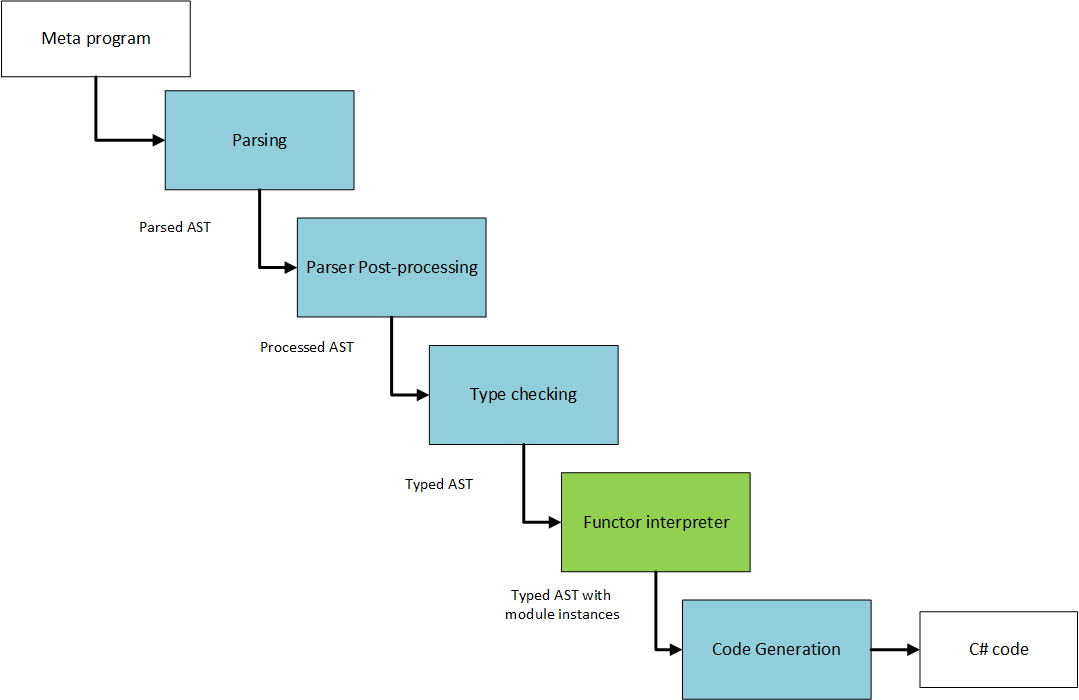
\includegraphics[width=\textwidth]{Figures/chapter_functors/compiler_architecture_functors}
	\caption{Compiler architecture with functor interpreter}
	\label{fig:ch_functors_compiler_architecture}
\end{figure}

\begin{figure}
	\centering
	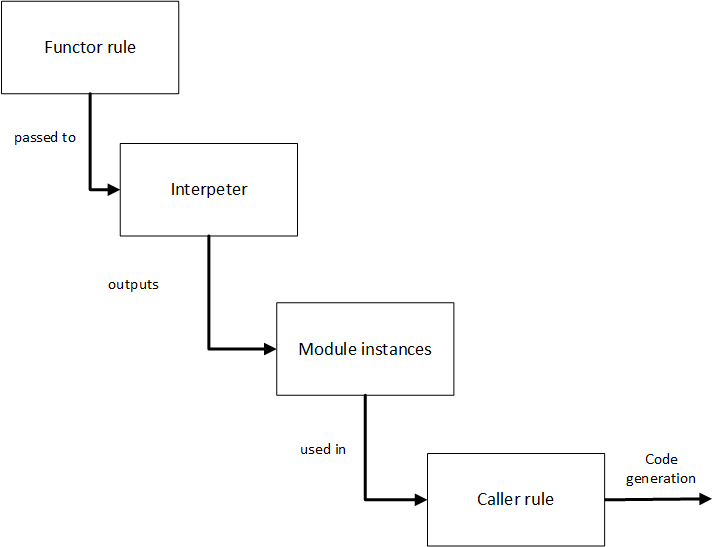
\includegraphics[width=\textwidth]{Figures/chapter_functors/functor_rule_processing}
	\caption{Functor processing}
	\label{fig:ch_functors_functor_processing}
\end{figure}

\section{Record implementation with modules}
\label{sec:ch_functors_record_implementation}
In Section \ref{subsec:ch_functors_inlining} we showed how Casanova entities can be expressed, at meta-language level, as a tuple of field names and values. We also showed that getters and setters always perform the same steps when looking up for the same field because the entity structure does not change at runtime. In this section we proceed to give an implementation based on functors to implement a Casanova entity. We refer to this implementation as ``Record'', since a Casanova entity is simply a record from the point of view of the data representation and since this solution works in general for any data structure that is isomorphic to a record. From now on we also use, as example, the physical body entity described in Section \ref{subsec:ch_functors_casanova_example}.

A module for records simply contains a functor that returns the type of the record. This functor, in general, can return any type since the type of the record can be ``customized'' and depends on the specific definition given by the programmer (thus it cannot be known beforehand). For this reason we use \textit{kind} as return type for this functor. The functor itself is parameterless since nothing is required to generate the type of a record.

\begin{lstlisting}
Module "Record" : Record {
  Functor "RecordType" : * }
\end{lstlisting}

The data representation of the record will be a tuple as shown in Section \ref{subsec:ch_functors_inlining}. For this purpose, we need two functors that are able to represent the type of a record in a recursive way with one being the type of an empty record (a record with no fields) and another a record field followed by the rest of the record representation. The functor for the empty record simply returns the type of the record module, while the functor to represent a record field takes as input a \texttt{string}, representing the name of the field, \textit{kind} because a record field can have any type, and a \texttt{Record} which represents all the other fields coming after the current one. 

\begin{lstlisting}
Functor "EmptyRecord" : Record
Functor "RecordField" => string => * => Record : Record
\end{lstlisting}

After declaring the functors necessary to build a record, we proceed to define their implementation in the form of rules. The functor for an empty record simply generates a module containing a function \texttt{cons}, that is the constructor for the record, that simply returns unit (because an empty record does not contain any field). Consistently, the functor \texttt{RecordType} implemented by the module will simply return \texttt{unit} as type. Note that a module instantiation must implement \textbf{at least} all the declarations of the module (like for an interface), but can add other declarations and implementations that are not shared by all the module instantiations. For example \texttt{cons} for an empty record is different than the one for a non-empty one.

\begin{lstlisting}
-------------------
EmptyRecord => Record {

  Func "cons" : unit
  
  ------------------
  RecordType => unit
  
  ------------------
  cons -> ()

}
\end{lstlisting}

A record field must be constructed through a functor that takes the field name, the type of the field, and the type of the rest of the record. This functor will construct the type of a record as a \texttt{Tuple}, where the first element is the type of the current field and the second the type of the rest of the record. The constructor of the record field will be a function that takes as input an argument of the type of the current field, a tuple representing the remaining part of the record and returns a tuple combining the current field and the rest of the record.

\begin{lstlisting}
------------------
RecordField name type r = Record {
  Func "cons" -> type -> r.RecordType : RecordType

  ---------------------------------------
  RecordType => Tuple[type,r.RecordType]

  -------------------
  cons x xs -> (x,xs)}
\end{lstlisting}

Consider now the physical body representation given above. We show how to use the functors we have just defined to build an instance of a physical body. First of all we defined a functor \texttt{PhysicalBodyType} that returns a \texttt{Record}.

\begin{lstlisting}
Functor "PhysicalBodyType" : Record
\end{lstlisting}

The final representation of the type that should be returned by\\ \texttt{PhysicalBodyType} is \texttt{Tuple[Vector2,Tuple[Vector2,unit]]} because the field \texttt{Position} and \texttt{Velocity} have type \texttt{Vector2}. Note that \texttt{Vector2} can be trivially implemented in Metacasanova as a tuple containing two floating point values. Here we use this type assuming that has already been defined above. The same appiles to \texttt{unit}, which can be defined as a meta-data with no arguments.

The rule to evaluate \texttt{PhysicalBodyType} will call in its premises \texttt{EmptyRecord} and \texttt{RecordField} to generate the type of the tuple appropriately:

\begin{lstlisting}
EmptyRecord => empty
RecordField "Velocity" Vector2 empty => velocity
RecordField "Position" Vector2 velocity => body
----------------------------
PhysicalBodyType => body
\end{lstlisting}

Let us now analyse in detail what the premises generate: the first premise will generate an instance of \texttt{EmptyRecord} and bind it to the variable \texttt{empty}. The instance of this module is parameterless and thus will always be the same every time the functor is invoked. The second premise will instantiate \texttt{RecordField} by using the string \texttt{"Velocity"} as field name, \texttt{Vector2} as field type, and \texttt{empty} as argument for the remaining part of the record (there is no other field after \texttt{Velocity} in the physical body). The instantiation of \texttt{RecordField} produces a rule for the functor \texttt{RecordType}. According to the definition above this functor generates \texttt{Tuple[type,r.RecordType]}. By replacing the argument values provided in the premise, we have that \texttt{type := Vector2} and \texttt{r := empty := EmptyRecord}. Thus \texttt{r.RecordType} uses the functor \texttt{RecordType} in the instance of \texttt{EmptyRecord} which returns the type \texttt{unit} (the call can be seen as \texttt{empty.RecordType}). Thus \texttt{r.RecordType} can be replaced with \texttt{unit}, thus leading to \texttt{Tuple[Vector2, unit]}. Thus the rule for the functor \texttt{RecordType} generated in the module returned by the second premise will be.

\begin{lstlisting}
-----------------------
RecordType => Tuple[Vector2,unit]
\end{lstlisting}

By replacing the argument variables with the values provided in the second premises we can also get the declaration and rule for \texttt{cons}. By replacing again \texttt{type} and \texttt{r.RecordType} as done before, we have that the declaration for \texttt{cons} in the current instance of the module becomes:

\begin{lstlisting}
Func "cons" -> Vector2 -> unit: Tuple[Vector2,unit]
\end{lstlisting}

\noindent
while the corresponding rule will be generated as

\begin{lstlisting}
--------------------
cons x xs -> (x,xs)
\end{lstlisting}

\noindent
The complete module instance will then look like:

\begin{lstlisting}
velocity := Record {
  Func "cons" -> Vector2 -> unit: Tuple[Vector2,unit]
  
  -----------------------
  RecordType => Tuple[Vector2,unit]
  
  --------------------
  cons x xs -> (x,xs)
}
\end{lstlisting}

The third premise calls \texttt{RecordField} with \texttt{name := "Position"}, \texttt{type := Vector2}, and \texttt{r := velocity}. Now in the definition of the \texttt{RecordField} module again the functor \texttt{RecordType} returns \texttt{Tuple[type,r.RecordType]}. Now \texttt{r.RecordType} can be rewritten as \texttt{velocity.RecordType} that returns (see the instantiation of \texttt{velocity} above) \texttt{Tuple[Vector2,unit]}. Thus\\ \texttt{RecordType} for the field \texttt{Position} will be instantiated as

\begin{lstlisting}
-----------------------
RecordType => Tuple[Vector2,Tuple[Vector2,unit]]
\end{lstlisting}

\noindent
Analogously the declaration of \texttt{cons} will be instantiated as

\begin{lstlisting}
Func "cons" -> Vector2 -> Tuple[Vector2,unit]: Tuple[Vector2,Tuple[Vector2,unit]]
\end{lstlisting}

\noindent
while its rule is the same. The full module instance will then be

\begin{lstlisting}
body := Record {
  Func "cons" -> Vector2 -> Tuple[Vector2,unit]: Tuple[Vector2,Tuple[Vector2,unit]]
  
  -----------------------
  RecordType => Tuple[Vector2,Tuple[Vector2,unit]
  
  --------------------
  cons x xs -> (x,xs)
}
\end{lstlisting}

\noindent
which is returned by the functor \texttt{PhysicalBodyType}. In order to build an instance of the physical body, we define a function that returns a value of type \texttt{PhysicalBodyType} (which in turn is simply\\ \texttt{Tuple[Vector2,Tuple[Vector2,unit]}):

\begin{lstlisting}
Func "PhysicalBody" : PhysicalBodyType.RecordType

-----------------------
PhysicalBody -> PhysicalBodyType.cons((10.0,10.0),((10.0,0.0),()))
\end{lstlisting}

\noindent
The rule creates a physical body in position $(10,10)$ moving at velocity $(10,0)$.\\

One of the main arguments in favour of using functors was that they should allow to embed the type system of the embedded language in the meta-type system of Metacasanova. This means that, at compile time, the meta-compiler should be able to detect a physical body that is constructed in the wrong way. Let us then assume that we define another function to build a physical body where the programmer uses a scalar for the velocity instead of a vector:

\begin{lstlisting}
Func "WrongPhysicalBody" : PhysicalBodyType.RecordType

-------------------------------------
WrongPhysicalBody ->  PhysicalBodyType.cons((10.0,10.0),(10.0,()))
\end{lstlisting}

\noindent
What happens is that \texttt{PhysicalBodyType.RecordType} is equal to\\ \texttt{Tuple[Vector2,Tuple[Vector2,unit]]}. At this point the type checker of Metacasanova will successfully match the first element of the tuple returned by the rule, which is correctly provided as a value of type \texttt{Vector2}, but will fail to check the second, which is \texttt{double} where it expects a \texttt{Vector2}. With the implementation based on dictionaries given in Section \ref{subsec:ch_mcnv_languages_casanova_semantics} this check happens dynamically at runtime by means of type rules defined in the meta-program, rather than statically like in this case.

\section{Using Modules and Functors in Metacasanova}
\label{subsec:record_implementation}
A module definition in Metacasanova is parametric with respect to types, in the sense that a module definition might contain some type parameters, and can be instantiated by passing the specific types to use. A module can contain the definition of data structures, functions, or functors.

\begin{lstlisting}
Module "Record" : Record {
  Functor "RecordType" : * }
\end{lstlisting}

The symbol \texttt{*} reads \textit{kind} and means that the functor might return any type. Indeed the type of a record (or class) in a programming language can be ``customized'' and depends on its specific definition, thus it is not possible to know it beforehand.

We the define two modules for the \textit{getter} and \textit{setter} of a field of a record. In this example, we use type parameters in the module definitions.

\begin{lstlisting}
Module "Getter" => (name : string) => (r : Record) {
  Functor "GetType" : *
  Func "get" -> (r.RecordType) : GetType }
  
Module "Setter" => (name : string) => (r : Record ) {
  Functor "SetType" : *
  Func "set" -> (r.RecordType) -> SetType : (r.RecordType) }
\end{lstlisting}

\noindent
These two modules respectively define a functor to retrieve the type of the record field, and a function to get or set its value. Note that in the function definitions \texttt{get} and \texttt{set} we are calling the functor of the \texttt{Record} module to generate the appropriate type for the signature. This is allowed, since the result of a functor is indeed a type.

A record meta-type (i.e. its representation at meta-language level) is recursively defined as a sequence of pairs $(field,type)$, whose termination is given by \texttt{EmptyField}. We thus define the following functors:

\begin{lstlisting}
Functor "EmptyRecord" : Record
Functor "RecordField" => string => * => Record : Record
\end{lstlisting}

\noindent
The first functor defines the end point of a record, which is simply a record without fields. The second functor defines a field as the pair mentioned above followed by other field definitions.

Moreover, we must define two functors that are able to dynamically build the \textit{getter} and \textit{setter} for the field.

\begin{lstlisting}
Functor "GetField" => string => Record : Getter
Functor "SetField" => string => Record : Setter
\end{lstlisting}

The behaviour of functor is expressed, as for normal functions, through a rule in the meta-program. A rule that evaluates a functor returns an instantiation of a module. Note that, inside a module instantiation, it is possible to define and implement functions other than those in the module definition, i.e. the module instantiation must implement \textit{at least} all the functors and functions of the definition. For instance, the following is the type rule instantiating the module for \texttt{EmptyRecord}:

\begin{lstlisting}
-------------------
EmptyRecord => Record {

  Func "cons" : unit

  ------------------
  RecordType => unit

  ------------------
  cons -> ()

}
\end{lstlisting}

\noindent
The function \texttt{cons} defines a constructor for the record, which, in the case of an empty record, returns nothing. The module instantiation for a record field evaluates as well \texttt{RecordType}, and has a different definition and evaluation of the function \texttt{cons} (because it is constructed in a different way):

\begin{lstlisting}
------------------
RecordField name type r = Record {
  Func "cons" -> type -> r.RecordType : RecordType
  
  ---------------------------------------
  RecordType => Tuple[type,r.RecordType]
  
  -------------------
  cons x xs -> (x,xs)} 
\end{lstlisting}

\noindent
Note that the return type of \texttt{cons} is to be intended as calling \texttt{RecordType} of the current module, so as it were \\ \texttt{this.RecordType}.
The getter of a field must be able to lookup the record data structure in search of the field and generate a function to get the value from it. For this reason, the functor instantiates two separate modules, depending on the name of the field that we are currently examining.

\begin{lstlisting}[caption = Module instantiations for getters, label = code:getters]
//Rule 1
name = fieldName
thisRecord := RecordField name type r
-----------------
GetField fieldName (RecordField name type r) => Getter name thisRecord {
  GetType => type
  
  ---------------
  get (x,xs) -> x}

//Rule 2
name <> fieldName
thisRecord := RecordField name type r
------------------
GetField fieldName (RecordField name type r) => Getter name type thisRecord{
  Functor "GetAnotherField" : Getter
  
  ---------------
  GetAnotherField => GetField fieldName r
  
  GetAnotherField => g
  ---------------
  GetType => g.GetType
  
  GetAnotherField => getter
  getter.get xs -> v
  -------------------
  get (x,xs) -> v }
\end{lstlisting}

\noindent
Analogously, the setter of a field instantiates two separate modules whether the current field is the one we want to set or not.

\begin{lstlisting}[caption = Module instantiations for setters, label = code:setters]
name = lt
thisRecord := RecordField name type r
----------
SetField lt (RecordField name type r) => Setter name thisRecord{
  
  -----------------
  SetType => type
  
  -------------------
  set (x,xs) v -> (v,xs)}

name <> lt
thisRecord := RecordField name type r
------------
SetField lt (RecordField name type r) => Setter name thisRecord{
  TypeFunc "SetAnotherField" : Setter
  
  -------------------------
  SetAnotherField => SetField lt r
  
  ----------------------------
  SetType => type
  
  SetAnotherField => setter
  setter.set xs v -> xs'
  ----------------------------------
  set (x,xs) v -> (x,xs') }
\end{lstlisting}

\section{Functor result inlining}
If a premise or a conclusion contains a call to a functor, this call is evaluated at compile time, rather than at runtime. Metacasanova has been extended with an interpreter which is able to evaluate the result of the functor calls. The behaviour of the interpreter follows the same logic explained when presenting the code generation steps in Section \ref{sec:code_generation}, thus here we do not present the details for brevity. When a rule outputs the instantiation of the module, the generated code will contain only rules of the modules which conclusion contains a function (i.e. functions that output values, not functors). In this way the generated code will contain a different version of those functions depending on the instantiation parameters of the module.

We now show how to use the implementation of the records given in Section \ref{subsec:record_implementation} for the physical body presented as a case study.
The definition of the record type for the physical body is done through a functor

\begin{lstlisting}
Functor "PhysicalBodyType" : Record

EmptyRecord => empty
RecordField "Velocity" Vector2 empty => velocity
RecordField "Position" Vector2 velocity => body
--------------------------
PhysicalBodyType => body
\end{lstlisting}

This rule is evaluated at compile time by the interpreter that generates one module for each field of the \texttt{PhysicalBody}, containing the constructor. For example, for the field \texttt{Velocity} the interpreter will generate\footnote{Note that here we give a high-level representation of the generated rules that are actually directly generated as C\# code.}

\begin{lstlisting}
Func "cons" -> Vector2 -> unit : Tuple[Vector2,unit]

------------------------
cons x xs -> (x,xs)
\end{lstlisting}

This because the functor will call the evaluation rule for \texttt{RecordField} with the argument \texttt{(Recordfield "Velocity" Vector2 (EmptyRecord))}. This rule generates the function \texttt{cons} by evaluating the result of the functors\\ \texttt{EmptyRecord.RecordType} and \texttt{RecordField.RecordType}, which respectively produce \texttt{unit} and \texttt{Tuple[Vector2,unit]}.

Instantiating a physical body will just require to build a function that returns the type of the physical body, which is obtained by calling the functor \texttt{PhysicalBodyType}.

\begin{lstlisting}
Func "PhysicalBody" : PhysicalBodyType.RecordType

-----------------------
PhysicalBody -> PhysicalBodyType.cons((Vector2.Zero,(Vector2.Zero,())))
\end{lstlisting}

Defining the setter and getter of a field, requires to use the functor \texttt{GetField} to generate the appropriate getter function. After the module has been correctly generated, we can use the getter for the field. For example, in order to get the position field, we use the following function.

\begin{lstlisting}
Func "getPos" -> PhysicalBodyType : Vector2

GetField "Position" PhysicalBodyType => getter
getter.get PhysicalBody -> p
-------------------------------
getPos -> p
\end{lstlisting}

The result of the premise \texttt{GetField} will be evaluated at compile time through the code in Listing \ref{code:getters} and will instantiate a module containing the following function definition and rule.

\begin{lstlisting}
Func "get" -> Tuple[Vector2,Tuple[Vector2,unit]] : Vector2

-------------------------
get (x,xs) -> x
\end{lstlisting}

\noindent
Note that the second premise of \texttt{getPos} will immediately call the \texttt{get} generated in this step. The case of \texttt{setPos} is analogous except the setter takes an additional argument.

Reading \texttt{Velocity} analogously uses a functor call to generate a getter:

\begin{lstlisting}
Func "getVel" -> PhysicalBodyType : Vector2

GetField "Velocity" PhysicalBodyType => getter
getter.get PhysicalBody -> p
-------------------------------
getVel -> p
\end{lstlisting}

\noindent
This time the functor will generate two different functions in two separate modules. The first time the record is processed, \texttt{Rule 2} in Listing \ref{code:getters} will be activated (because the first field in the Record is \texttt{Position}). This rule will instantiate an additional module when evaluating the functor call in its premise, which in turn is able to get the \texttt{Velocity} field. The rule for \texttt{get} in the first module will contain in its premise a call to  \texttt{get} of the second module.

\begin{lstlisting}
//Code for module1
Func "get" -> Tuple[Vector2,Tuple[Vector2,unit]] : Vector2

module2.get xs -> v
-------------------------
get (x,xs) -> v

//Code for module2 generated by evaluating the functor in the premise of Rule 2
Func "get" -> Tuple[Vector2,unit] : Vector2

------------------
get (x,xs) -> x
\end{lstlisting}

We want to point out that this optimization has been presented on the specific case of records, but can be generalized for any situations where you would use a symbol table. Indeed any symbol table can be expressed with the representation above as a sequence of pair where the first item is the value of the current variable, and the second item is the continuation of the symbol table.

\section{Evaluation}
An extensive evaluation of Casanova implemented in Metacasanova, which we omit for brevity, can be found in \cite{DiGiacomo2017}. The implementation of Casanova operational semantics in Metacasanova is almost 5 times shorter than the corresponding F\# implementation in the hard-coded compiler. In addition to Casanova, we have implemented a subset of the C language called C-{}-. This language supports \texttt{if-then-else}, \texttt{while-loop}, and \texttt{for} statements, as well as local scoping of variables. The total length of the language definition in Metacasanova is 353 lines of code. The corresponding C\# code to implement the operational semantics of the language is 3123 lines, thus the code reduction with Metacasanova is roughly 8.84 times. For comparison, in Table \ref{tab:cmm} it is possible to see the code length to implement three different statements, both in Metacasanova and C\#. We tested C-{}- against Python by computing the average running time to compute the factorial of a number. C-{}- results to be 50 times slower than Python. This result is worse than what we obtained with Casanova, because in order to emulate the interruptible rule mechanism of Casanova in Python you must rely on coroutines that are slower than a program containing simple statements. Moreover, we tested the performance improvement of the optimization using Functors to represent records against the standard one using dynamic symbol tables. The test was run using records with a number of fields ranging from 1 to 10 and updating from 10000 to 1000000 instances of such records. In Table \ref{tab:functors}, we can see that the optimization using Functors leads to a performance increase on average of about 11 times, with peaks of 30 times. The gain increases with the number of fields, thus Functors are particularly effective for records with high number of fields. Figure \ref{fig:chart} shows a chart of the overall performance of the two techniques (the data points are taken from Table \ref{tab:functors}). The horizontal axis contains the amount of fields per record, while the vertical axis contains the number of records that are being updated. We can see that the performance of the dynamic table degrades considerably when increasing the number of fields, and that the higher the amount of records is, the steeper the curve is. On the other hand, the performance of the implementation with Functors is almost constant, regardless of the amount of fields or records that are being updated. Moreover, note that the performance of the dynamic table is improved by the fact that we are using a dictionary implemented in .NET, which can access the entries in $O(\log n)$. If the symbol table were represented as a meta-data structure in the language the performance would be even worse, since it would have to be encoded as a list of pairs with the field name and its value, and its manipulation would be affected by the evaluation rules that should implement this behaviour. Furthermore, the dynamic lookup should be done also to ensure that the types of the record fields are used consistently (for example to prevent that a record is constructed with incompatible values for its fields), while using the functors in Metacasanova embeds the type system of the language in the meta-type system, whose type safety is checked at compile-time rather than at runtime, and this contributes to further increase the performance.

\begin{table}	
	\caption{Running time with the functor optimization and the dynamic table with 10000, 100000, and 1000000 records.}
	\begin{tabular}{|c|c|c|c|}
		\hline
		\textbf{FIELDS}& \textbf{Functors (ms)}&\textbf{Dynamic Table (ms)} & \textbf{Gain}\\ \hline
		1&	1.00E-05&	5.00E-06&	0.50\\ \hline
		2&	9.00E-06&	1.30E-05&	1.44\\ \hline
		3&	9.00E-06&	2.70E-05&	3.00\\ \hline
		4&	9.00E-06&	4.50E-05&	5.00\\ \hline
		5&	9.00E-06&	7.00E-05&	7.78\\ \hline
		6&	9.00E-06&	9.90E-05&	11.00\\ \hline
		7&	9.00E-06&	1.33E-04&	14.78\\ \hline
		8&	9.00E-06&	1.75E-04&	19.44\\ \hline
		9&	9.00E-06&	2.20E-04&	24.44\\ \hline
		10&	9.00E-06&	2.70E-04&	30.00\\ \hline
		\multicolumn{2}{c|}{} & \textbf{Average gain} & 11.74\\ \cline{3-4}			
	\end{tabular}
	
	\vspace{0.15cm}
	\begin{tabular}{|c|c|c|c|}
		\hline
		\textbf{FIELDS}& \textbf{Functors (ms)}&\textbf{Dynamic Table (ms)} & \textbf{Gain}\\ \hline
		1&	9.60E-05&	6.30E-05&	0.66\\ \hline
		2&	9.40E-05&	1.59E-04&	1.69\\ \hline
		3&	9.50E-05&	3.04E-04&	3.20\\ \hline
		4&	9.60E-05&	5.03E-04&	5.24\\ \hline
		5&	9.60E-05&	7.52E-04&	7.83\\ \hline
		6&	9.60E-05&	1.05E-03&	10.95\\ \hline
		7&	9.70E-05&	1.41E-03&	14.57\\ \hline
		8&	9.80E-05&	1.82E-03&	18.59\\ \hline
		9&	9.90E-05&	2.29E-03&	23.17\\ \hline
		10&	1.00E-04&	2.81E-03&	28.05\\ \hline
		\multicolumn{2}{c|}{} & \textbf{Average gain} & 11.39\\ \cline{3-4}						
	\end{tabular}
	
	\vspace{0.15cm}
	\begin{tabular}{|c|c|c|c|}
		\hline
		\textbf{FIELDS}& \textbf{Functors (ms)}&\textbf{Dynamic Table (ms)} & \textbf{Gain}\\ \hline
		1&	9.47E-04&	7.29E-04&	0.77\\ \hline
		2&	9.51E-04&	1.78E-03&	1.87\\ \hline
		3&	9.50E-04&	3.33E-03&	3.51\\ \hline
		4&	9.60E-04&	5.43E-03&	5.66\\ \hline
		5&	9.65E-04&	8.03E-03&	8.32\\ \hline
		6&	9.71E-04&	1.11E-02&	11.44\\ \hline
		7&	9.75E-04&	1.47E-02&	15.12\\ \hline
		8&	9.82E-04&	1.89E-02&	19.28\\ \hline
		9&	9.92E-04&	2.37E-02&	23.86\\ \hline
		10&	1.00E-03&	2.87E-02&	28.62\\ \hline
		\multicolumn{2}{c|}{} & \textbf{Average gain} & 11.84\\ \cline{3-4}						
	\end{tabular}
	\label{tab:functors}
\end{table}

\begin{figure}
	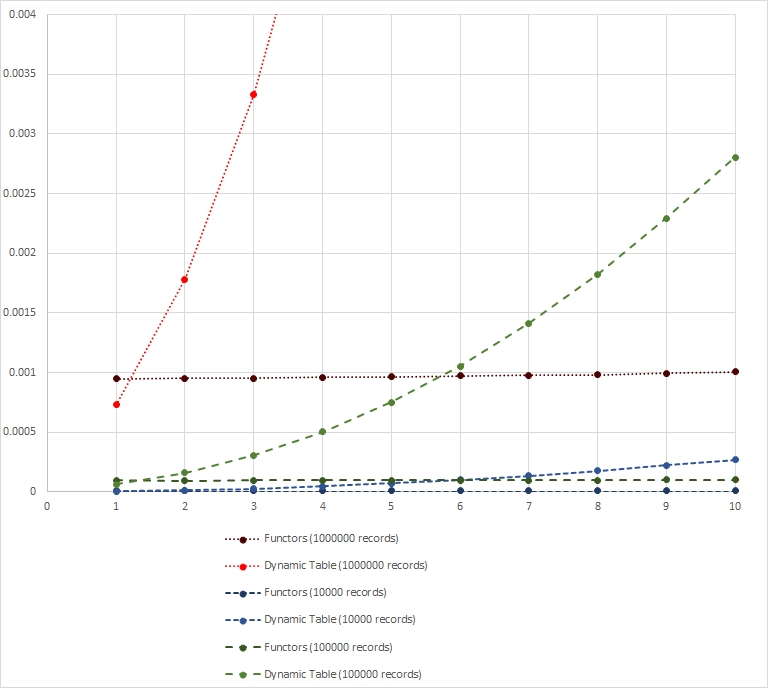
\includegraphics[width = \columnwidth]{Figures/functor_chart.jpg}
	\caption{Execution time of the different memory models}
	\label{fig:chart}
\end{figure}
